% Cover letter using letter.cls
\documentclass{article} % Uses 10pt
%\usepackage{helvetica} % uses helvetica postscript font (download helvetica.sty)
%\usepackage{newcent}   % uses new century schoolbook postscript font 
\usepackage[utf8]{inputenc}       % allow Latin1 characters
\usepackage{graphicx}
% the following commands control the margins:
%\topmargin=-1in    % Make letterhead start about 1 inch from top of page 
%\textheight=8.5in    % text height can be bigger for a longer letter
%\oddsidemargin=0pt   % leftmargin is 1 inch
%\textwidth=6.5in     % textwidth of 6.5in leaves 1 inch for right margin
\title{Implementierung eines Temperatur und Luftfeuchtigkeits Sensornetzwerks für den nEDM Experiment Aufbau\\-\\IDP Kurzbeschreibung}
\author{Wenwen Chen, Rainer Schönberger}
\begin{document}
\maketitle
\section*{Das nEDM Experiment}
\subsection*{Überblick}
Nach dem Standardmodell der Teilchenphysik wird derzeit angenommen, dass
Neutronen durch elektroschwache Wechselwirkung ein elektrisches Dipolmoment
in der Größenordnung von etwa $10^{-32}e\cdot cm$ haben. Eine Erweiterung des
Standardmodells wird ein Dipolmoment des Neutrons bereits im Bereich zwischen
$10^{-26}e\cdot cm$ und $10^{-28}e\cdot cm$ vorhergesagt. Derzeit liegt das
Limit für Messungen des Dipolmoments bei ca. $10^{-26}e\cdot cm$\\
Das Neutron EDM Experiment an der TUM versucht deshalb die Messgenauigkeit so
weit zu steigern, damit die oben genannte Theorie entweder belegt oder
widerlegt werden kann.\\
Um dies zu erreichen, werden spinpolarisierte ultrakalte Neutronen (UCN) in
zwei Kammern in einer hochgradig kontrollierten und magnetisch abgeschirmten
Umgebung gefüllt. Dort wird dann eine Spinpräzessionsmessung nach Ramsey
durchgeführt, mit welcher Informationen über das elektrische Dipolmoment des
Neutrons gewonnen werden.
\subsection*{Notwendigkeit der Umgebungsmessung}
\section*{Die Vorlesung ``Particle Physics with Neutrons''}
\section*{Unser Projekt}
\subsection*{Überblick}
- Anforderungsanalyse
- Recherche nach passender Hardware
- Aufbau der Hardware
- Implementieren einer Software lösung
- Installation des Sensornetzwerks im Experimentaufbau
\subsection*{Meilensteine}
Der vorgesehene Zeitplan und Aufgabenaufteilung sind folgendes:
\begin{center}
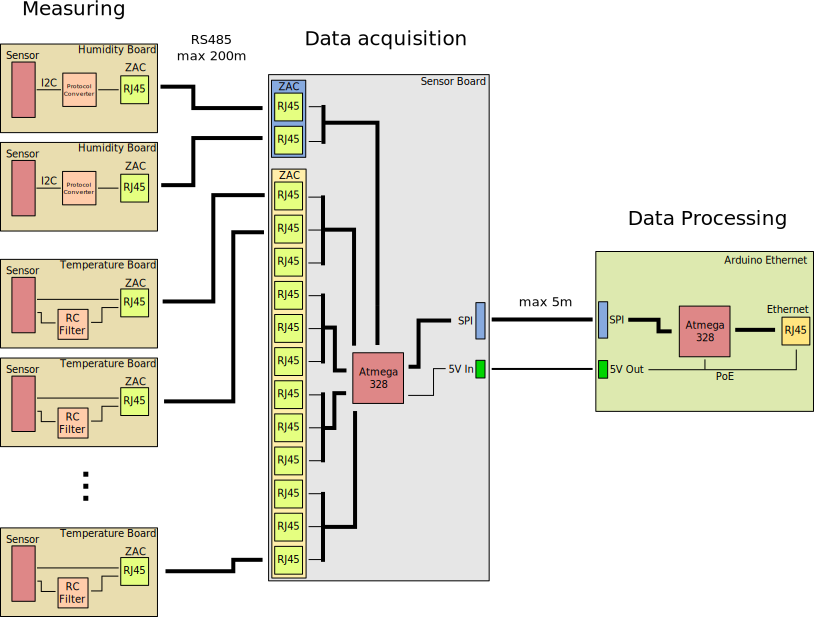
\includegraphics[]{plan.pdf}
\end{center}
\end{document}
